\section{构建CPA安全的密码}

在这一节中,我们描述了一些构建针对选择明文攻击是语义安全的密码的方法。正如我们在例 \ref{exmp:5-1} 中讨论的,任何这样的密码都必须是概率性的。在 \ref{subsec:5-4-1} 小节中,我们将首先介绍一种将任何语义安全的密码与伪随机函数(PRF)相结合的通用构造,其中,PRF 被用于生成``一次性"密钥。接下来,在 \ref{subsec:5-4-2} 小节中,我们会提出一种 \ref{subsec:4-4-4} 小节中介绍的\emph{计数器模式}密码的概率性变体。虽然这个方案可以基于任何PRF,但在实践中,我们通常使用一个分组密码来实例化这个PRF。最后,在 \ref{subsec:5-4-3} 小节,我们将介绍一种名为\emph{密码分组链接(CBC)}的模式,它能使用分组密码构建新的密码。

后两种构造,即计数器模式和CBC模式,被称为\emph{区块密码的操作模式}。我们已经在 \ref{subsec:4-1-4} 小节中介绍过另一种操作模式,即\emph{电子密码本(ECB)}模式。然而,由于这种操作模式缺乏安全性,它现在已经很少被实际使用。还有其他提供CPA安全性的操作模式,我们会在练习中进行更详细地讨论。


\subsection{一种通用混合构造}\label{subsec:5-4-1}

在本小节中,我们将展示如何使用适当的 PRF 将任何语义安全的密码 $\mathcal{E}=(E,D)$ 转化为 CPA 安全的密码 $\mathcal{E}'$。

其基本思想是这样的。$\mathcal{E}'$ 的密钥是 $F$ 的密钥 $k'$。为了加密一条消息 $m$,我们选取一个 $F$ 的随机输入 $x$,并通过计算 $k\leftarrow F(k',x)$ 得到 $\mathcal{E}$ 的密钥 $k$。然后,我们用密钥 $k$ 对 $m$ 进行加密:$c\overset{\rm R}\leftarrow E(k,m)$。密文为 $c':=(x,c)$。请注意,我们需要把 $x$ 作为 $c'$ 的一部分,这是为了便于解密:解密算法首先计算 $k\leftarrow F(k',x)$ 以得到密钥 $k$,然后通过计算 $m\leftarrow D(k,c)$ 恢复 $m$。

为了使上述过程起作用,$F$ 的输出空间必须与 $\mathcal{E}$ 的密钥空间相匹配。同时,$F$ 的输入空间必须是超多项式的,这是为了使得产生两个相同 $x$  值的概率可忽略不计。

下面我们讨论细节。令 $\mathcal{E}=(E,D)$ 是一个定义在 $(\mathcal{K},\mathcal{M},\mathcal{C})$ 上的密码,$F$ 是一个定义在 $(\mathcal{K}',\mathcal{X},\mathcal{K})$ 上的 PRF。也就是说,$F$ 的输出空间应该等于 $\mathcal{E}$ 的密钥空间。我们定义一个 $(\mathcal{K}',\mathcal{M},\mathcal{X}\times\mathcal{C})$ 上的新密码 $\mathcal{E}'=(E',D')$ 如下:
\begin{itemize}
	\item 对于 $k'\in\mathcal{K}'$ 和 $m\in\mathcal{M}$,我们定义:
	
	\hspace*{20pt} $E'(k',m):=\quad x\overset{\rm R}\leftarrow\mathcal{X},\ k\leftarrow F(k',x),\ c\overset{\rm R}\leftarrow E(k,m)$\\
	\hspace*{88pt} 输出 $(x,c)$;
	\item 对于 $k'\in\mathcal{K}'$ 和 $c'=(x,c)\in\mathcal{X}\times\mathcal{C}$,我们定义:
	
	\hspace*{20pt} $D'(k',c'):=\quad k\leftarrow F(k',x),\ m\leftarrow D(k,c)$\\
	\hspace*{88pt} 输出 $m$。
\end{itemize}    

不难验证,$\mathcal{E}'$ 确实是一个密码,而且是我们看到的第一个\emph{概率性}密码。

\begin{example}\label{exmp:5-2}
在证明 $\mathcal{E}'$ 的 CPA 安全性之前,让我们先看看这个构造的实际情况。假设 $\mathcal{E}$ 是一个一次性密码本,即 $E(k,m):=k\oplus m$,其中 $\mathcal{K}=\mathcal{M}=\mathcal{C}=\{0,1\}^L$。将上面的通用混合构造应用于一次性密码本,就能得到以下的一种非常流行的密码 $\mathcal{E}_0=(E_0,D_0)$:
\begin{itemize}
	\item 对于 $k'\in\mathcal{K}'$ 和 $m\in\mathcal{M}$,定义:
	
	\hspace*{20pt} $E_0(k',m):=\quad x\overset{\rm R}\leftarrow\mathcal{X}$,输出 $(x,\ F(k',x)\oplus m)$
	\item 对于 $k'\in\mathcal{K}'$ 和 $c'=(x,c)\in\mathcal{X}\times\mathcal{C}$,定义:
	
	\hspace*{20pt} $D_0(k',c'):=\quad$ 输出 $F'(k',x)\oplus c$
\end{itemize}
该密码的 CPA 安全性来自于通用混合构造 $\mathcal{E}'$ 的 CPA 安全性,而后者将在下面的定理 \ref{theo:5-2} 中得到证明。
\end{example}

\begin{theorem}\label{theo:5-2}
如果 $F$ 是一个安全的 PRF,$\mathcal{E}$ 是一个语义安全的密码,并且 $N:=|\mathcal{X}|$ 是超多项式的,则上面描述的密码构造 $\mathcal{E}'$ 是一个 CPA 安全的密码。
\begin{quote}
特别地,对于每个像攻击游戏 \ref{game:5-2} 的比特猜测版本那样攻击 $\mathcal{E}'$ 的 CPA 对手 $\mathcal{A}$,假设它最多能向其挑战者发起 $Q$ 次查询,则必然存在一个像攻击游戏 \ref{game:4-2} 中那样攻击 $F$ 的 PRF 对手 $\mathcal{B}_F$,和一个像攻击游戏 \ref{game:2-1} 的比特猜测版本那样攻击 $\mathcal{E}$ 的 SS 对手 $\mathcal{B}_\mathcal{E}$,其中 $\mathcal{B}_F$ 和 $\mathcal{B}_\mathcal{E}$ 都是围绕 $\mathcal{A}$ 的基本包装器,满足:
\end{quote}
\begin{equation}\label{eq:5-5}
{\rm CPA}\mathsf{adv}[\mathcal{A},\mathcal{E}']\leq
\frac{Q^2}{N}+2\cdot{\rm PRF}\mathsf{adv}[\mathcal{B}_F,F]+Q\cdot{\rm SS}\mathsf{adv}[\mathcal{B}_\mathcal{E},\mathcal{E}]
\end{equation}
\end{theorem}

\begin{proof}[证明思路]
首先,利用 $F$ 是一个 PRF 的假设,我们可以有效地用一个真随机函数代替 $F$。其次,利用 $N$ 是超多项式的假设,我们认为任意两个 $x$ 值相同的概率都可忽略不计。而在本场景中,挑战者的密钥都是独立生成的,所以挑战者实际上扮演与攻击游戏 \ref{game:5-1} 中的挑战者相同的角色。那么,由定理 \ref{theo:5-1} 即可证明定理 \ref{theo:5-2}。
\end{proof}

\begin{proof}
假设 $\mathcal{A}$ 是一个有效 CPA 对手,它像攻击游戏 \ref{game:5-2} 中那样攻击 $\mathcal{E}'$。假设 $\mathcal{A}$ 最多能够对其挑战者发起 $Q$ 次查询。现在,假设 $F$ 是一个安全 PRF,$N$ 是超多项式的,$\mathcal{E}$ 是语义安全的,我们的目标是证明 ${\rm CPA}\mathsf{adv}[\mathcal{A},\mathcal{E}']$ 可以忽略不计。

我们不妨使用CPA攻击游戏和SS攻击游戏的比特猜测版本。我们想要证明,对于有效对手 $\mathcal{B}_F$ 和 $\mathcal{B}_\mathcal{E}$,有:
\begin{equation}\label{eq:5-6}
{\rm CPA}\mathsf{adv}^*[\mathcal{A},\mathcal{E}']\leq
\frac{Q^2}{2N}+{\rm PRF}\mathsf{adv}[\mathcal{B}_F,F]+Q\cdot{\rm SS}\mathsf{adv}^*[\mathcal{B}_\mathcal{E},\mathcal{E}]
\end{equation}
那么根据定理 \ref{theo:2-10} 和式 \ref{eq:2-11},我们就能够证明式 \ref{eq:5-5} 成立。

该证明的基本策略如下。首先,我们定义游戏 $0$ 为 $\mathcal{A}$ 和挑战者在攻击游戏 \ref{game:5-2} 的比特猜测版本中就 $\mathcal{E}'$ 进行的游戏。此外,我们再定义几个个游戏:游戏$1$,游戏$2$ 和游戏$3$,其中每一个都是在 $\mathcal{A}$ 和不同的挑战者之间进行的。另外,正如我们将要看到的,游戏 $3$ 就等同于就 $\mathcal{E}$ 所进行的攻击游戏 \ref{game:5-1} 的比特猜测版本。在这些游戏中,$b$ 表示挑战者选择的随机比特,而 $\hat b$ 表示 $\mathcal{A}$ 输出的比特。此外,对于 $j = 1,\dots,3$,我们定义 $W_j$ 为游戏 $j$ 中 $\hat{b}=b$ 成立的事件。我们将表明,对于 $j = 1,\dots,3$,$|\Pr[W_j]-\Pr[W_{j-1}]|$ 的值可忽略不计;此外,由于我们假设 $\mathcal{E}$ 是语义安全的,根据定理 \ref	{theo:5-1},$|\Pr[W_3]-{1}/{2}|$ 也可忽略不计。由此,我们可以看出${\rm CPA}\mathsf{adv}^*[\mathcal{A},\mathcal{E}']:=|\Pr[W_0]-{1}/{2}|$也可忽略不计。

\vspace{5pt}

\noindent\textbf{游戏$\mathbf{0}$}。
我们先对游戏 $0$ 中的挑战者进行详细描述,这对我们的证明是很方便的:

\vspace{5pt}

\hspace*{5pt} 选取 $b\overset{\rm R}\leftarrow\{0,1\}$\\
\hspace*{26pt} 选取 $k'\overset{\rm R}\leftarrow\mathcal{K}'$\\
\hspace*{26pt} 对于 $i=1,\dots,Q$:\\
\hspace*{50pt} 选取 $x_i\overset{\rm R}\leftarrow\mathcal{X}$\\
\hspace*{50pt} 计算 $k_i\leftarrow F'(k',x_i)$\\
\hspace*{26pt} 当收到第 $i$ 个查询 $(m_{i0},m_{i1})\in\mathcal{M}^2$ 时:\\
\hspace*{50pt} 计算 $c_i\overset{\rm R}\leftarrow E(k_i,m_{ib})$\\
\hspace*{50pt} 将 $(x_i,c_i)$ 发送给对手。

\vspace{5pt}

根据构造,我们有:
\begin{equation}\label{eq:5-7}
{\rm CPA}\mathsf{adv}^*[\mathcal{A},\mathcal{E}']= |\Pr[W_0]-{1}/{2}|
\end{equation}


\noindent\textbf{游戏$\mathbf{1}$}。
接下来,我们打出我们的``PRF牌",用一个真随机函数 $f\in{\rm Funs}[\mathcal{X},\mathcal{K}]$ 代替 $F(k',\cdot)$。在该游戏中,挑战者看起来是这样的:

\vspace{5pt}

\hspace*{5pt} 选取 $b\overset{\rm R}\leftarrow\{0,1\}$\\
\hspace*{26pt} 选取 $f'\overset{\rm R}\leftarrow{\rm Funs}[\mathcal{X},\mathcal{K}]$\\
\hspace*{26pt} 对于 $i=1,\dots,Q$:\\
\hspace*{50pt} 选取 $x_i\overset{\rm R}\leftarrow\mathcal{X}$\\
\hspace*{47pt} \colorbox{gray!50}{计算 $k_i\leftarrow f(x_i)$}\\
\hspace*{26pt} 当收到第 $i$ 个查询 $(m_{i0},m_{i1})\in\mathcal{M}^2$ 时:\\
\hspace*{50pt} 计算 $c_i\overset{\rm R}\leftarrow E(k_i,m_{ib})$\\
\hspace*{50pt} 将 $(x_i,c_i)$ 发送给对手。

\vspace{5pt}

我们声称:
\begin{equation}\label{eq:5-8}
|\Pr[W_1]-\Pr[W_0]|={\rm PRF}\mathsf{adv}[\mathcal{B}_F,F]
\end{equation}
其中 $\mathcal{B}_F$ 是一个有效 PRF 对手;此外,由于我们假设 $F$ 是一个安全 PRF,所以 ${\rm PRF}\mathsf{adv}[\mathcal{B}_F,F]$ 一定可忽略不计。

游戏 $0$ 和游戏 $1$ 的语法很自然地为 $\mathcal{B}_F$ 的设计提供了灵感。如果 $f\in{\rm Funs}[\mathcal{X},\mathcal{K}]$ 表示挑战者在攻击游戏 \ref{game:4-2} 中就 $F$ 所选择的函数,则对手 $\mathcal{B}_F$ 的运行逻辑如下:

\vspace{5pt}

\hspace*{5pt} 首先,$\mathcal{B}_F$ 进行以下计算:

\vspace{5pt}

\hspace*{28.5pt} 选取 $b\overset{\rm R}\leftarrow\{0,1\}$\\
\hspace*{50pt} 对于 $i=1,\dots,Q$:\\
\hspace*{50pt} 选取 $x_i\overset{\rm R}\leftarrow\mathcal{X}$\\
\hspace*{50pt} 计算 $k_i\leftarrow f(x_i)$

\vspace{8pt}

\hspace*{5pt} 这里,$\mathcal{B}_F$ 用 $x_i$ 向自己的挑战者发起查询,并获得 $f(x_i)$ 的值。

\vspace{3pt}

\hspace*{5pt} 接下来,$\mathcal{B}_F$ 扮演 $\mathcal{A}$ 的挑战者;特别地,当 $\mathcal{A}$ 发起它的第 $i$ 个查询 $(m_{i0},m_{i1})$ 时,对手 $\mathcal{B}_F$ 计算:
	\[c_i\overset{\rm R}\leftarrow E(k_i,m_{ib})\]
\hspace*{26pt} 并将 $(x_i,c_i)$ 发送给 $\mathcal{A}$。

\vspace{5pt}
    
\hspace*{5pt} 最终,$\mathcal{A}$ 停机并输出一个比特 $\hat{b}$,$\mathcal{B}_F$ 也同时停机,如果 $\hat{b}=b$,$\mathcal{B}_F$ 输出 $1$,否则输出 $0$。

\vspace{5pt}

\noindent
对手 $\mathcal{B}_F$ 的工作逻辑可参见图 \ref{fig:5-1}。如之前一样,$\delta(x,y)$ 在 $x=y$ 时等于 $1$,否则等于 $0$。

\begin{figure}
  \centering
  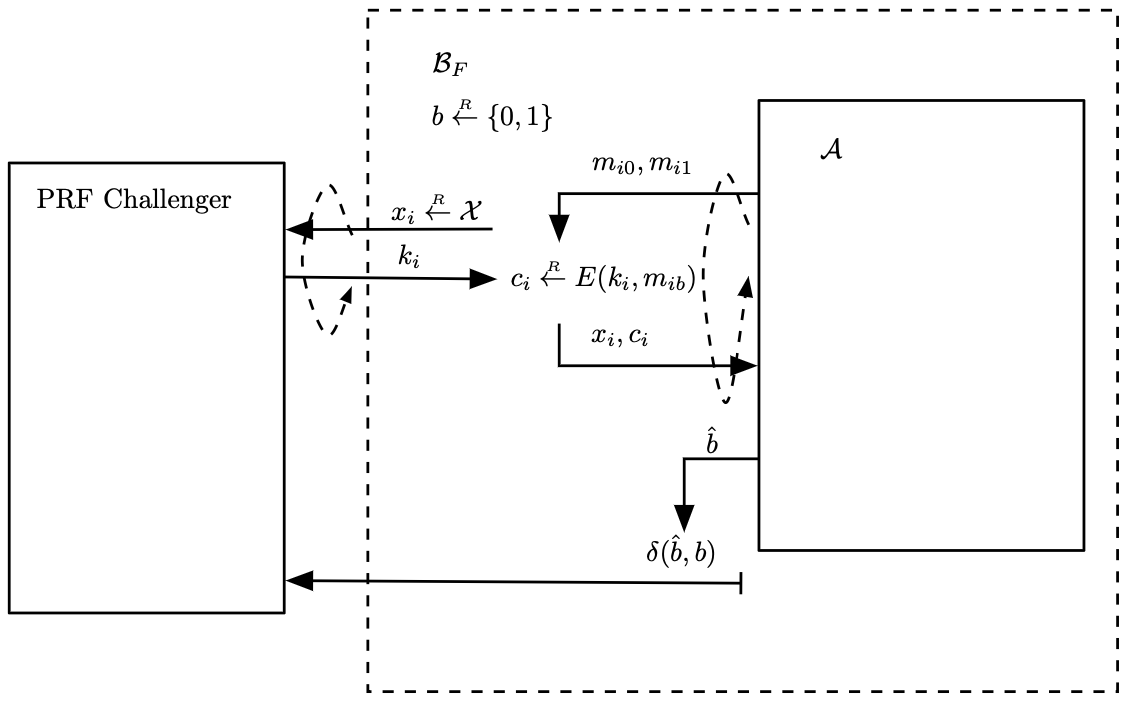
\includegraphics[width=0.8\linewidth]{figures/chapter5/fig1.png}
  \caption{定理 \ref{theo:5-2} 的证明中的对手 $\mathcal{B}_F$}
  \label{fig:5-1}
\end{figure}

\vspace{5pt}

\noindent\textbf{游戏$\mathbf{2}$}。
接下来,我们使用我们的``忠实的侏儒"的思路(见 \ref{subsec:4-4-2} 小节)来实现随机函数 $f$。我们的``侏儒"必须跟踪 $f$ 的输入,并检测相同的输入是否被使用了两次。在下面的逻辑中,我们的``侏儒"使用一个真随机值作为 $k_i$ 的``默认"值,但如果有必要的话,这个值也可以被覆写,就像标有 ($*$) 的那一行所示:

\vspace{5pt}

\hspace*{5pt} 选取 $b\overset{\rm R}\leftarrow\{0,1\}$\\
\hspace*{26pt} 对于 $i=1,\dots,Q$:\\
\hspace*{50pt} 选取 $x_i\overset{\rm R}\leftarrow\mathcal{X}$\\
\hspace*{50pt} 计算 $k_i\leftarrow\mathcal{K}$\\
\hspace*{3pt} ($*$)
\hspace*{26.5pt} 如果存在某个 $j<i$ 使得 $x_i=x_j$,就令 $k_i\leftarrow k_j$\\
\hspace*{26pt} 当收到第 $i$ 个查询 $(m_{i0},m_{i1})\in\mathcal{M}^2$ 时:\\
\hspace*{50pt} 计算 $c_i\overset{\rm R}\leftarrow E(k_i,m_{ib})$\\
\hspace*{50pt} 将 $(x_i,c_i)$ 发送给对手。

\vspace{5pt}

\noindent
由于这是对随机函数 $f$ 的忠实实现,我们有:
\begin{equation}\label{eq:5-9}
\Pr[W_2]=\Pr[W_1]
\end{equation}

\noindent\textbf{游戏$\mathbf{3}$}。
接下来,我们让我们的侏儒变得``健忘",只需要丢掉上一个游戏中标有 ($*$) 的那一行:

\vspace{5pt}

\hspace*{5pt} 选取 $b\overset{\rm R}\leftarrow\{0,1\}$\\
\hspace*{26pt} 对于 $i=1,\dots,Q$:\\
\hspace*{50pt} 选取 $x_i\overset{\rm R}\leftarrow\mathcal{X}$\\
\hspace*{50pt} 计算 $k_i\leftarrow\mathcal{K}$\\
\hspace*{26pt} 当收到第 $i$ 个查询 $(m_{i0},m_{i1})\in\mathcal{M}^2$ 时:\\
\hspace*{50pt} 计算 $c_i\overset{\rm R}\leftarrow E(k_i,m_{ib})$\\
\hspace*{50pt} 将 $(x_i,c_i)$ 发送给对手。

\vspace{5pt}

为了分析 $|\Pr[W_3]-\Pr[W_2]|$ 的值,我们使用差分引理(定理 \ref{theo:4-7})。为此,我们将游戏 $2$ 和游戏 $3$ 视为运行在相同的基础概率空间上:对手和挑战者所做的随机选择在两个游戏中都是相同的,仅有的不同是挑战者计算应答的规则。特别地,两个游戏中的变量 $x_i$ 都是相同的。我们定义 $Z$ 为存在 $i\neq j$ 使得 $x_i=x_j$ 成立的事件。显然,除非 $Z$ 发生,否则游戏 $2$ 和游戏 $3$ 的流程是相同的;特别是,当且仅当 $W_3\land\bar{Z}$ 发生时,$W_2\land\bar{Z}$ 才会发生。因此,基于差分引理,我们有:
\begin{equation}\label{eq:5-10}
|\Pr[W_3]-\Pr[W_2]|\leq\Pr[Z]
\end{equation}
此外,不难发现:
\begin{equation}\label{eq:5-11}
\Pr[Z]\leq\frac{Q^2}{2N}
\end{equation}
这是因为 $Z$ 是小于 ${Q^2}/{2}$ 个事件的联合,其中每个事件发生的概率都是 ${1}/{N}$。

注意到,在游戏 $3$ 中,每条消息都使用独立的密钥 $k_i$ 来加密。所以接下来,我们打``语义安全牌",声称:
\begin{equation}\label{eq:5-12}
|\Pr[W_3]-{1}/{2}|={\rm MSS}\mathsf{adv}^*[\mathcal{\bar{B}}_\mathcal{E}, \mathcal{E}]
\end{equation}
其中,$\mathcal{\bar{B}}_\mathcal{E}$ 是一个有效对手,它就 $\mathcal{E}$ 进行攻击游戏 \ref{game:5-1} 的比特猜测版本,在该游戏中最多向其挑战者发起 $Q$ 次查询。

游戏 $3$ 语法很自然地为 $\mathcal{\bar{B}}_\mathcal{E}$ 的设计提供了灵感,它的工作方式如下:
\begin{quote}
$\mathcal{\bar{B}}_\mathcal{E}$ 扮演 $\mathcal{A}$ 的挑战者,在收到 $\mathcal{A}$ 的第 $i$ 个查询 $(m_{i0},m_{i1})$ 时,将 $(m_{i0},m_{i1})$ 提交给自己的挑战者,并得到一个密文 $c_i\in\mathcal{C}$。然后 $\mathcal{\bar{B}}_\mathcal{E}$ 从 $\mathcal{X}$ 中随机选择 $x_i$,并将 $(x_i,c_i)$ 发送给 $\mathcal{A}$ 作为对后者查询的应答。

当 $\mathcal{A}$ 最终输出一比特 $\hat{b}$ 时,$\mathcal{\bar{B}}_\mathcal{E}$ 也输出这个比特。
\end{quote}
对手 $\mathcal{\bar{B}}_\mathcal{E}$ 的工作原理见图 \ref{fig:5-2}。

\begin{figure}
  \centering
  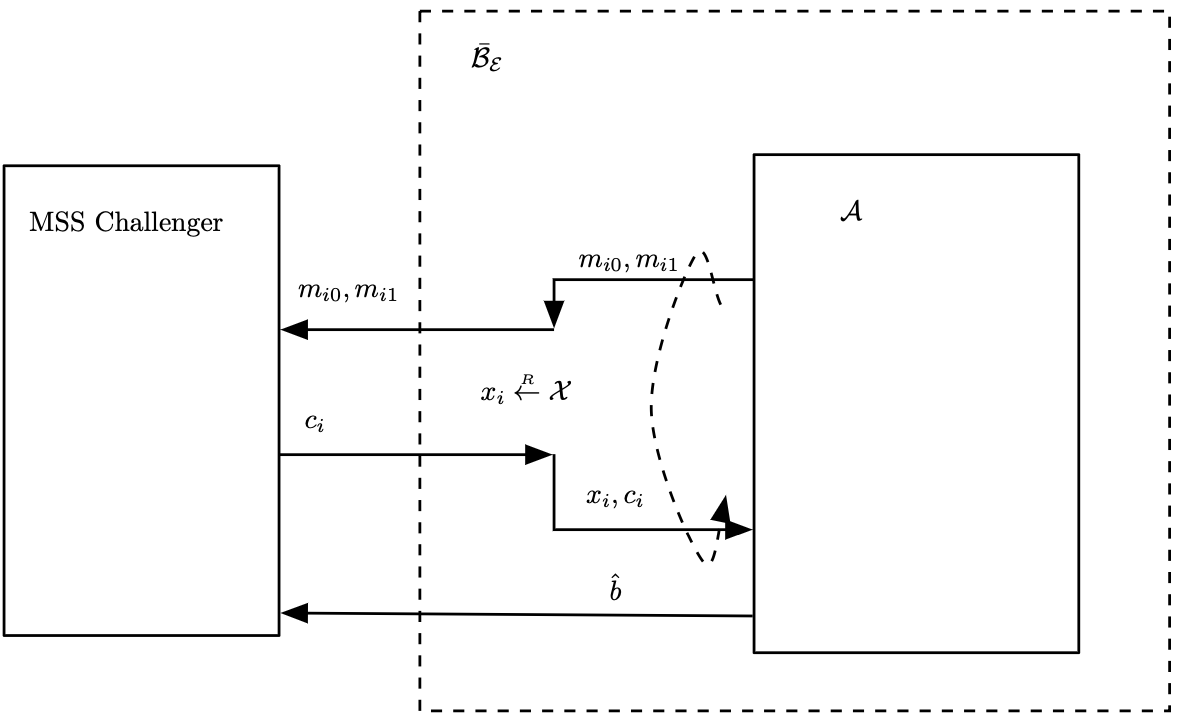
\includegraphics[width=0.8\linewidth]{figures/chapter5/fig2.png}
  \caption{定理 \ref{theo:5-2} 的证明中的对手 $\mathcal{\bar{B}}_\mathcal{E}$}
  \label{fig:5-2}
\end{figure}

从构造(和式 \ref{eq:2-11})可以看出,式 \ref{eq:5-12} 显然成立。此外,根据定理 \ref{theo:5-1} 和式 \ref{eq:5-1},我们有:
\begin{equation}\label{eq:5-13}
{\rm MSS}\mathsf{adv}^*[\mathcal{\bar{B}}_\mathcal{E}, \mathcal{E}]=Q\cdot{\rm SS}\mathsf{adv}^*[\mathcal{B}_\mathcal{E},\mathcal{E}]
\end{equation}
其中 $\mathcal{B}_\mathcal{E}$ 是一个有效对手,它就 $\mathcal{E}$ 进行攻击游戏 \ref{game:2-1} 的比特猜测版本。

将式 \ref{eq:5-7} 到式 \ref{eq:5-13} 相结合,我们就可以得到式 \ref{eq:5-6}。另外,我们可以发现,$\mathcal{B}_F$ 和 $\mathcal{B}_\mathcal{E}$ 的运行时间与 $\mathcal{A}$ 的运行时间大致相同;事实上,它们都是围绕 $\mathcal{A}$ 的基本包装器,无论 $\mathcal{A}$ 是否是有效的,式 \ref{eq:5-5} 都是成立的。
\end{proof}

虽然上面的证明有点长,但我们希望读者认识到它实际上是很自然的,而且所有的步骤都相当容易掌握。另外,这个证明还说明了在设计一个安全证明时,我们如何引入一个以上的安全假设,并将安全证明设计成一连串的游戏。

\begin{remark}\label{remark:5-2}
我们简单提一下,即使构造中所使用的 PRF $F$ 只是弱安全的(见定义 \ref{def:4-3}),定理 \ref{theo:5-2} 中的混合构造 $\mathcal{E}'$ 仍然是 CPA 安全的。为了在这个较弱的假设下证明定理 \ref{theo:5-2},注意到,在游戏 $0$ 和游戏 $1$ 中,挑战者只在 $\mathcal{X}$ 中的\emph{随机}点上评估 PRF。因此,即使 $F$ 只是弱安全的,对手区分游戏 $0$ 和 $1$ 的优势也是可忽略不计的。
\end{remark}

\subsection{随机化计数器模式}\label{subsec:5-4-2}

我们可以直接从一个安全的 PRF 中构建一个 CPA 安全的密码,如下所示。假设 $F$ 是一个定义在 $(\mathcal{K},\mathcal{X},\mathcal{Y})$ 上的 PRF。我们假设 $\mathcal{X}=\{0,\dots,N-1\}$,并且 $\mathcal{Y}=\{0,1\}^n$。

对于任意多项式边界的 $\ell\geq1$,我们定义一个密码 $\mathcal{E}=(E,D)$,其密钥空间为 $\mathcal{K}$,消息空间为 $\mathcal{Y}^{\leq\ell}$,密文空间为 $\mathcal{X}\times\mathcal{Y}^{\leq\ell}$,如下所示:
\begin{itemize}
	\item 对于 $k\in\mathcal{K}$ 和 $m\in\mathcal{Y}^{\leq\ell}$,记 $v:=|m|$,我们定义:
	
	\hspace*{20pt} $E(k,m):=$\\
	\hspace*{50pt} 选取 $x\overset{\rm R}\leftarrow\mathcal{X}$\\
	\hspace*{50pt} 按如下方式计算 $c\in\mathcal{Y}^v$:\\
	\hspace*{75pt} 对于 $j=0,1,\dots,v-1$:\\
	\hspace*{100pt} 令 $c[j]\leftarrow F(k,\,x+j\;\mathrm{mod}\;N)\oplus m[j]$\\
	\hspace*{50pt} 输出 $(x,c)$;
	\item 对于 $k\in\mathcal{K}$ 和 $c'=(x,c)\in\mathcal{X}\times\mathcal{Y}^{\leq\ell}$,记 $v:=|c|$,我们定义:
	
	\hspace*{20pt} $D(k,c'):=$\\
	\hspace*{50pt} 按如下方式计算 $m\in\mathcal{Y}^v$:\\
	\hspace*{75pt} 对于 $j=0,1,\dots,v-1$:\\
	\hspace*{100pt} 令 $m[j]\leftarrow F(k,\,x+j\;\mathrm{mod}\;N)\oplus c[j]$\\
	\hspace*{50pt} 输出 $m$。
\end{itemize}

这个密码构造很像我们在 \ref{subsec:4-4-4} 小节中介绍的从 PRF 中建立一个 PRG,进而得到的流密码。不同的是,我们现在不再向 $F$ 输入固定序列以派生出密钥流,而是从一个随机起点开始,递增地来获得 $F$ 的输入序列。密文中的 $x$ 部分通常被称为\textbf{初始值 (initial value, IV)}。

在实践中,我们通常使用分组密码的加密函数来实现这里的 $F$,其中 $\mathcal{X}=\mathcal{Y}=\{0,1\}^n$。我们很自然地可以将 $n$ 比特的序列视为 $\{0,\dots,2^n-1\}$ 范围内的一个整数。碰巧的是,在这个构造中,我们根本就不需要分组密码的解密函数。关于这种模式的说明,可见图 \ref{fig:5-3}。

不难验证 $\mathcal{E}$ 确实是一个(概率性)密码。另外,需要注意的是,$\mathcal{E}$ 的消息空间是可变长的,如果想要使用攻击游戏 \ref{game:5-2} 定义的 CPA 安全性,消息 $m\in\mathcal{Y}^{\leq\ell}$ 的长度应当是其自然长度 $|m|$。

\begin{figure}[p!]
  \centering
  \subfigure[加密]{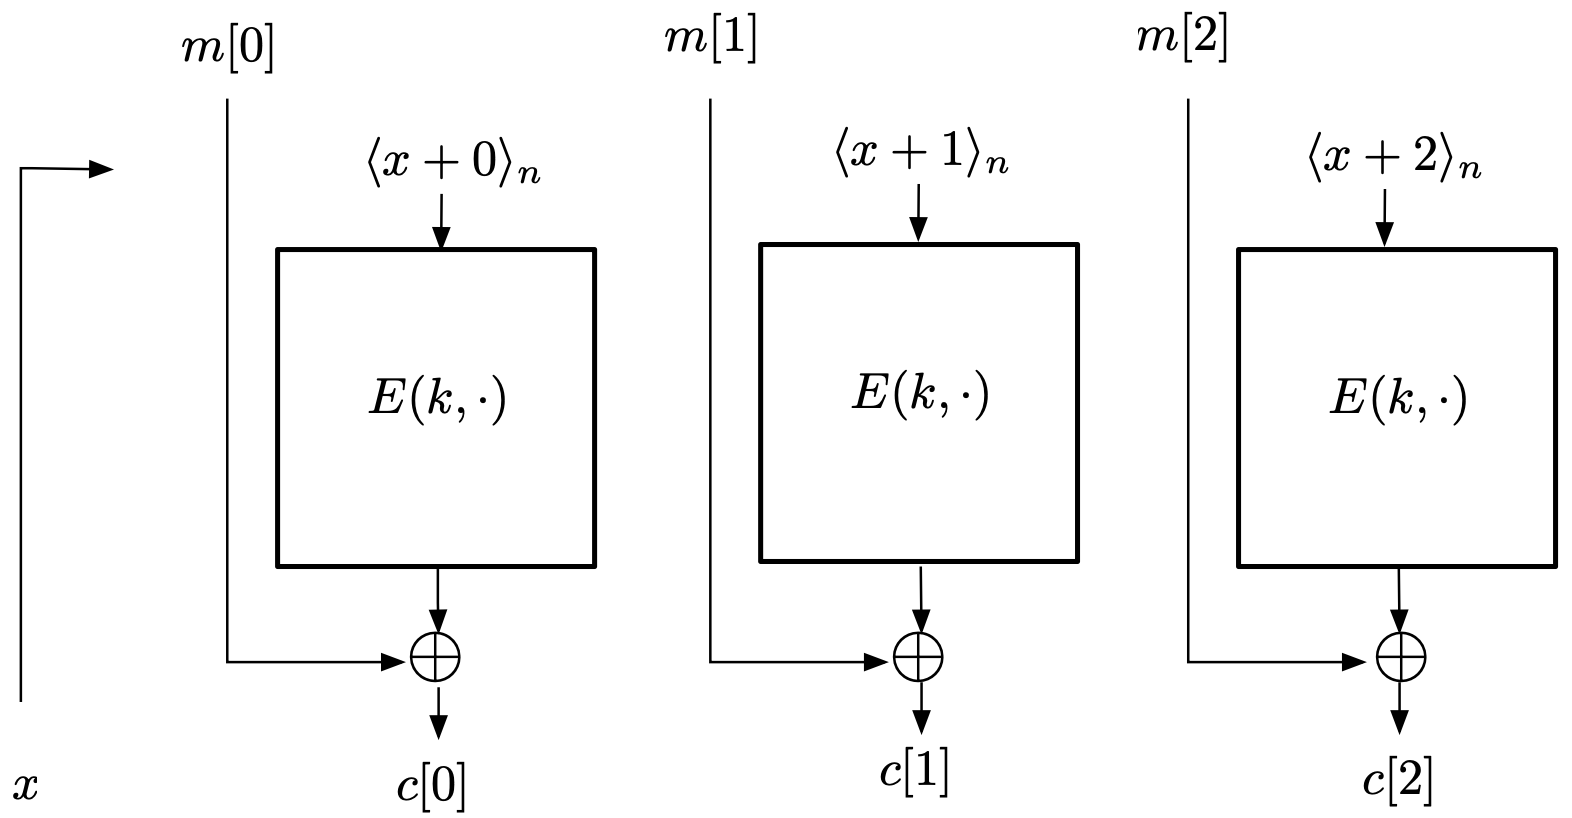
\includegraphics[width=0.65\linewidth]{figures/chapter5/fig3-a.png}}

  \subfigure[解密]{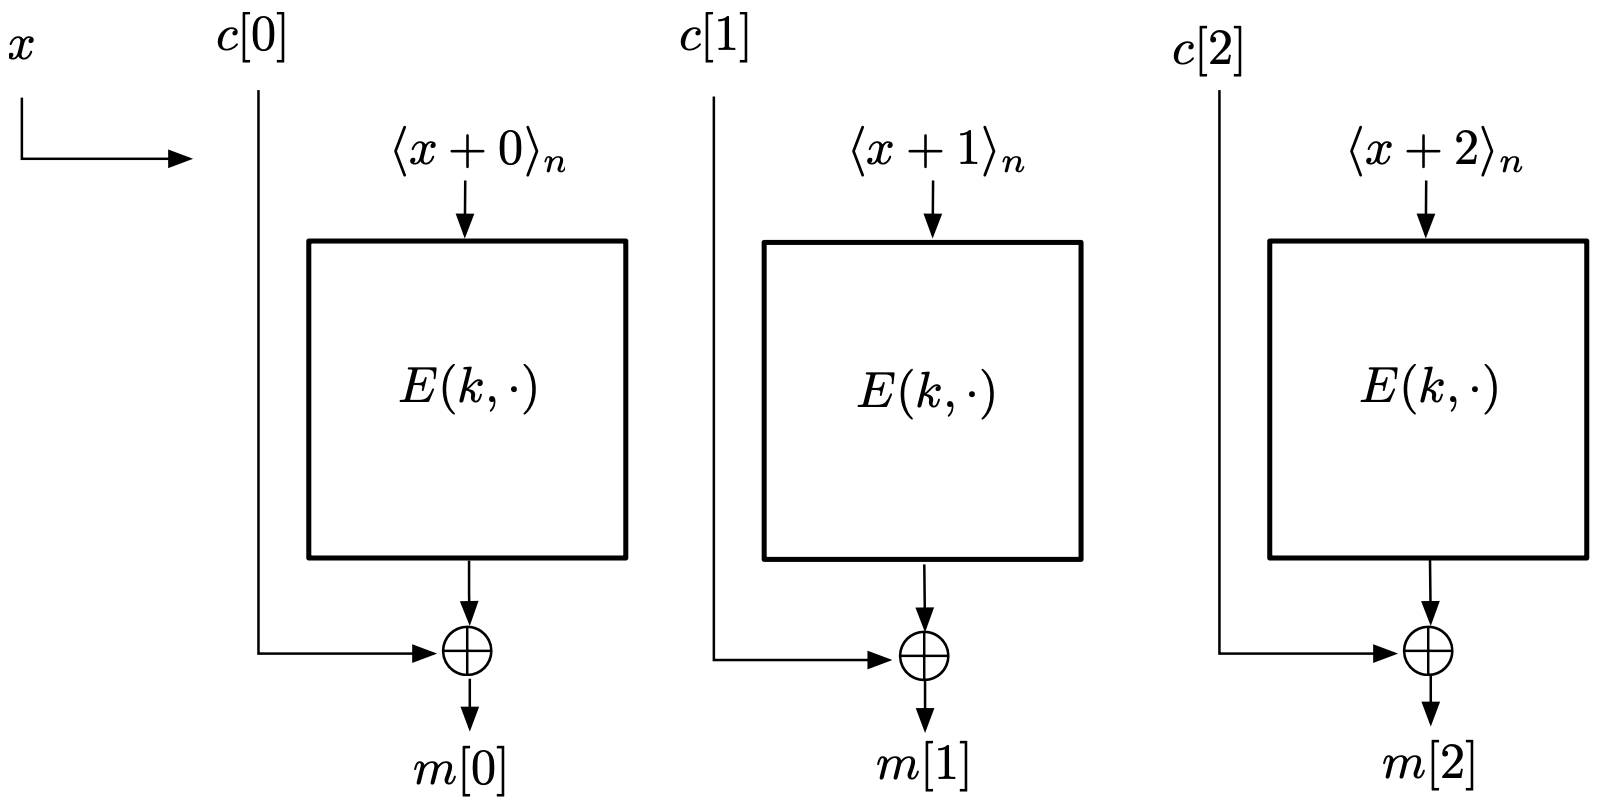
\includegraphics[width=0.65\linewidth]{figures/chapter5/fig3-b.png}}
  \caption{随机化计数器模式($v=3$)}
  \label{fig:5-3}
\end{figure}

\begin{theorem}\label{theo:5-3}
如果 $F$ 是一个安全的 PRF,并且 $N$ 是超多项式的,那么对于任何多项式约束的 $\ell\geq1$,上面描述的密码 $\mathcal{E}$ 都是一个 CPA 安全的密码。
\begin{quote}
特别地,对于每一个如攻击游戏 \ref{game:5-2} 中那样攻击 $\mathcal{E}$ 的 CPA 对手 $\mathcal{A}$,如果它最多能向其挑战者发起 $Q$ 次查询,则必然存在一个如攻击游戏 \ref{game:4-2} 中那样攻击 $F$ 的 PRF 对手 $\mathcal{B}$,其中 $\mathcal{B}$ 是一个围绕 $\mathcal{A}$ 的基本包装器,满足:
\end{quote}
\begin{equation}\label{eq:5-14}
{\rm CPA}\mathsf{adv}[\mathcal{A},\mathcal{E}]\leq\frac{2Q^2\ell}{N}+2\cdot{\rm PRF\mathsf{adv}}[\mathcal{B},F]
\end{equation}
\end{theorem}

\begin{proof}[证明思路]
假设我们从一个就 $\mathcal{E}$ 进行攻击游戏的对手开始。首先,利用 $F$ 是一个安全 PRF 的假设,我们可以有效地用一个真随机函数 $f$ 代替 $F$。其次,利用 $N$ 是超多项式的假设,以及每个 IV 都是随机选择的这一事实,我们可以认为,挑战者两次使用同一输入值评估 $f$ 的概率是可忽略不计的。但在这里,挑战者实际上是用一个独立的一次性密码本加密每条消息的,因此我们可以得出结论,对手在原始的 CPA 攻击游戏中的优势也是可忽略不计的。
\end{proof}

\begin{proof}
令 $\mathcal{A}$ 是一个有效对手,它就 $\mathcal{E}$ 进行攻击游戏 \ref{game:5-2},并且在该游戏中最多可以向其挑战者发起 $Q$ 次查询。我们想证明,如果 $F$ 是一个安全的 PRF,且 $N$ 是超多项式的,则 ${\rm CPA}\mathsf{adv}[\mathcal{A},\mathcal{E}]$ 可忽略不计。

不妨使用攻击游戏 \ref{game:5-2} 的比特猜测版本。我们需要证明,对于一个有效对手 $\mathcal{B}$,有:
\begin{equation}\label{eq:5-15}
{\rm CPA}\mathsf{adv}^*[\mathcal{A}, \mathcal{E}]\leq\frac{Q^2\ell}{N}+{\rm PRF\mathsf{adv}}[\mathcal{B},F]
\end{equation}
那么式 \ref{eq:5-14} 就可由式 \ref{eq:5-4} 得到。

这个证明的基本策略如下。首先,我们将游戏 $0$ 定义为 $\mathcal{A}$ 与其挑战者在攻击游戏 \ref{game:5-2} 的比特猜测版本中就 $\mathcal{E}$ 所进行的游戏。然后,我们再定义另外几个个游戏:游戏 $1$,游戏$2$ 和游戏 $3$。这些游戏都是在 $\mathcal{A}$ 和不同的挑战者之间进行的。在每个游戏中,我们用 $b$ 表示挑战者随机选择的比特,用 $\hat b$ 表示 $\mathcal{A}$ 输出的比特。我们想要证明,对于 $j = 1,\dots,3$,$|\Pr[W_j]-\Pr[W_{j-1}]|$ 的值都可忽略不计;此外,$\Pr[W_3]={1}/{2}$ 是显然成立的,继而我们可以得到 ${\rm CPA}\mathsf{adv}^*[\mathcal{A}, \mathcal{E}]:=|\Pr[W_0]-{1}/{2}|$ 也可忽略不计。

\vspace{5pt}

\noindent\textbf{游戏$\mathbf{0}$}。
我们可以将游戏 $0$ 中的挑战者描述如下:

\vspace{5pt}

\hspace*{5pt} 选取 $b\overset{\rm R}\leftarrow\{0,1\}$\\
\hspace*{26pt} 选取 $k'\overset{\rm R}\leftarrow\mathcal{K}$\\
\hspace*{26pt} 对于 $i=1,\dots,Q$:\\
\hspace*{50pt} 选取 $x_i\overset{\rm R}\leftarrow\mathcal{X}$\\
\hspace*{50pt} 对于 $j=0,\dots,\ell-1$:\\
\hspace*{75pt} 计算 $x_{ij}'\leftarrow x_i+j\mod N$\\
\hspace*{75pt} 计算 $y_{ij}\leftarrow F(k,x_{ij}')$\\
\hspace*{26pt} 当收到第 $i$ 个查询 $(m_{i0},m_{i1})$ 时,记 $v_i:=|m_{i0}|=|m_{i1}|$:\\
\hspace*{50pt} 按如下方法计算 $c_i\in\mathcal{Y}^{v_i}$:\\
\hspace*{75pt} 对于 $j=0,\dots,v_i-1$:\\
\hspace*{100pt} 计算 $c_i[j]\leftarrow y_{ij}\oplus m_{ib}[j]$\\
\hspace*{50pt} 将 $(x_i,c_i)$ 发送给对手。

\vspace{5pt}

根据构造,我们有:
\begin{equation}\label{eq:5-16}
{\rm CPA}\mathsf{adv}^*[\mathcal{A},\mathcal{E}]= |\Pr[W_0]-{1}/{2}|
\end{equation}

\noindent\textbf{游戏$\mathbf{1}$}。
接下来,我们打出我们的``PRF牌",用一个真随机函数 $f\in{\rm Funs}[\mathcal{X},\mathcal{Y}]$ 代替 $F(k,\cdot)$。在该游戏中,挑战者看起来是这样的:

\vspace{5pt}

\hspace*{5pt} 选取 $b\overset{\rm R}\leftarrow\{0,1\}$\\
\hspace*{26pt} 选取 $f\overset{\rm R}\leftarrow{\rm Funs}[\mathcal{X},\mathcal{Y}]$\\
\hspace*{26pt} 对于 $i=1,\dots,Q$:\\
\hspace*{50pt} 选取 $x_i\overset{\rm R}\leftarrow\mathcal{X}$\\
\hspace*{50pt} 对于 $j=0,\dots,\ell-1$:\\
\hspace*{75pt} 计算 $x_{ij}'\leftarrow x_i+j\mod N$\\
\hspace*{75pt} 计算 $y_{ij}\leftarrow f(x_{ij}')$\\
\hspace*{26pt} $\dots$

\vspace{5pt}

我们省略了挑战者的一部分代码,因为这些部分在所有游戏中都不会改变。我们声称:
\begin{equation}\label{eq:5-17}
|\Pr[W_1]-\Pr[W_0]|={\rm PRF}\mathsf{adv}[\mathcal{B},F]
\end{equation}
其中 $\mathcal{B}$ 是一个有效 PRF 对手;此外,由于我们假设 $F$ 是一个安全的 PRF,所以 ${\rm PRF}\mathsf{adv}[\mathcal{B},F]$ 一定是可忽略不计的。希望这(目前)已经是一个常规的论证,我们把具体的论证细节留给读者自行完成。

\vspace{5pt}

\noindent\textbf{游戏$\mathbf{2}$}。
接下来,我们用我们的``忠实的侏儒"的思路来实现随机函数 $f$。在描述我们的挑战者在这个游戏中的逻辑时,我们需要对索引数对 $(i,j)$ 使用标准词法排序;也就是说,当且仅当:
\[
i'<i
\quad\text{or}\quad
i'=i
\;\text{and}\;
j'<j
\]
时,我们记 $(i',j')<(i,j)$。在下面的逻辑中,我们的``侏儒"使用一个真随机值作为每个 $y_{ij}$ 的``默认"值,但如果有必要的话,这个值也可以被覆写,就像标有 ($*$) 的那一行所示:

\vspace{5pt}

\hspace*{5pt} 选取 $b\overset{\rm R}\leftarrow\{0,1\}$\\
\hspace*{26pt} 对于 $i=1,\dots,Q$:\\
\hspace*{50pt} 选取 $x_i\overset{\rm R}\leftarrow\mathcal{X}$\\
\hspace*{50pt} 对于 $j=0,\dots,\ell-1$:\\
\hspace*{75pt} 计算 $x_{ij}'\leftarrow x_i+j\mod N$\\
\hspace*{75pt} 计算 $y_{ij}\overset{\rm R}\leftarrow\mathcal{Y}$\\
\hspace*{3pt} ($*$)
\hspace*{51pt} 如果存在某个 $(i',j')<(i,j)$ 使得 $x_{ij}'=x_{i'j'}'$,则令 $y_{ij}\leftarrow y_{i'j'}$\\
\hspace*{26pt} $\dots$

\vspace{5pt}

由于这是对随机函数 $f$ 的忠实实现,我们有:
\begin{equation}\label{eq:5-18}
\Pr[W_2]=\Pr[W_1]
\end{equation}

\noindent\textbf{游戏$\mathbf{3}$}。
接下来,我们让我们的侏儒变得``健忘",只需要丢掉上一个游戏中标有 ($*$) 的那一行:

\vspace{5pt}

\hspace*{5pt} 选取 $b\overset{\rm R}\leftarrow\{0,1\}$\\
\hspace*{26pt} 对于 $i=1,\dots,Q$:\\
\hspace*{50pt} 选取 $x_i\overset{\rm R}\leftarrow\mathcal{X}$\\
\hspace*{50pt} 对于 $j=0,\dots,\ell-1$:\\
\hspace*{75pt} 计算 $x_{ij}'\leftarrow x_i+j\mod N$\\
\hspace*{75pt} 计算 $y_{ij}\overset{\rm R}\leftarrow\mathcal{Y}$\\
\hspace*{26pt} $\dots$

\vspace{5pt}

为了分析 $|\Pr[W_3]-\Pr[W_2]|$ 的值,我们使用差分引理(定理 \ref{theo:4-7})。为此,我们将游戏 $2$ 和游戏 $3$ 视为运行在相同的基础概率空间上:对手和挑战者所做的随机选择在两个游戏中都是相同的,仅有的不同是挑战者计算应答的规则。特别地,两个游戏中的变量 $x_{ij}'$ 都是相同的。我们定义 $Z$ 为存在某个 $(i',j')\neq(i,j)$ 使得 $x_{ij}'=x_{i'j'}'$ 成立的事件。显然,除非 $Z$ 发生,否则游戏 $2$ 和游戏 $3$ 的流程是相同的;特别是,当且仅当 $W_3\land\bar{Z}$ 发生时,$W_2\land\bar{Z}$ 才会发生。因此,基于差分引理,我们有:
\begin{equation}\label{eq:5-19}
|\Pr[W_3]-\Pr[W_2]|\leq\Pr[Z]
\end{equation}

我们声称:
\begin{equation}\label{eq:5-20}
\Pr[Z]\leq\frac{Q^2\ell}{N}
\end{equation}
为了证明这一声称,我们可以假设 $N\geq2\ell$(这一点无论如何都应该是普遍成立的,因为我们假设 $\ell	$ 是多项式边界的,$N$ 是超多项式的)。观察到,对于满足 $i\neq i'$ 的索引对 $i$ 和 $i'$,当且仅当:
\[
\{x_i,\dots,x_i+\ell-1\}
\;\cap\;
\{x_{i'},\dots,x_{i'}+\ell-1\}
\neq\varnothing
\]
成立时,事件 $Z$ 才会发生(算术运算是模 $N$ 的)。考虑任意固定的满足上述要求的一个数对 $(i,i')$。当以任意固定的 $x_i$ 为条件时,$x_i'$ 均匀分布在 $\{0,\dots,N-1\}$ 上,并且当且仅当:
\[
x_{i'}\in\{x_i+j\,:\,-\ell+1\leq j\leq\ell-1\}
\]
时,这些区间才会有重叠,这发生的概率是 ${2\ell-1}/{N}$,这样,由于我们有 ${Q(Q-1)}/{2}$ 种方法选择 $i$ 和 $i'$,所以式 \ref{eq:5-20} 成立。

最后,观察到,在游戏 $3$ 中,$y_{ij}$ 的值均匀独立分布在 $\mathcal{Y}$ 上,因此挑战者本质上是使用独立的一次性密码本来加密的。特别是,我们很容易看到,对手在这个游戏中的输出与 $b$ 无关,因此有:
\begin{equation}\label{eq:5-21}
\Pr[W_3]={1}/{2}
\end{equation}

将式 \ref{eq:5-16} 和 \ref{eq:5-21} 相结合,我们就可以得到式 \ref{eq:5-15},这就证明了本定理。
\end{proof}

\begin{remark}\label{remark:5-3}
我们可以把随机化计数器模式看作是 \ref{subsec:5-4-1} 小节中的通用混合构造的一个特例。参见联系 5.5。
\end{remark}

\subsubsection{案例研究:AES 计数器模式}

IPsec 协议使用 RFC 3686 中规定的 AES 计数器模式的一个特殊的变体。回顾一下,AES 使用 $128$ 比特长的分组。RFC 3686 不为每个消息随机挑选一个 $128$ 比特的 IV,而是按以下方式挑选 IV:
\begin{itemize}
	\item 最高的 $32$ 个有效比特是在生成密钥时随机选取的,并且在密钥的有效期内是固定的。这 $32$ 比特会用于所有使用该密钥加密的消息。
	\item 随后的 $64$ 比特是从 $\{0,1\}^{64}$ 中随机选出的。
	\item 最低的 $32$ 个有效比特均被置为 $1$。
\end{itemize}
通过这种方法产生的 $128$ 比特 IV 被用作计数器的初始值。在加密消息时,每加密一个消息分组,IV 的最低 $32$ 个有效比特就会递增一次。因此,可以加密的最大消息长度是 $2^{32}$ 个 AES 分组,即 $2^{36}$ 个字节。

通过这种 IV 的选择,解密者知道 IV 的最高 $32$ 个有效比特和最低 $32$ 个有效比特。因此,只有中间 $64$ 比特的 IV 需要和密文一起发送。

通过套用定理 \ref{theo:5-3} 的证明方法,我们同样可以证明这样选择 IV 是安全的。这种方法比随机选取 $128$ 位 IV 的微弱优势在于,本方法所产生的密文要更短一些。一个随机的 IV 会迫使加密器在密文中包含所有的 $128$ 个比特,而使用 RFC 3686 的方法,只需要 $64$ 比特,这就使密文缩小了 $8$ 个字节。

\subsection{密码分组链接模式}\label{subsec:5-4-3}

历史上的一个很重要的加密方法是在密码分组链接 (cipher block chaining, CBC) 模式下使用一个分组密码。这种方法被用在了 TLS 协议的旧版本中(比如 TLS 1.0)。它劣于下一节将要讨论的计数器模式加密。

令 $\mathcal{E}=(E,D)$ 是一个定义在 $(\mathcal{K},\mathcal{X})$ 上的分组密码,其中 $\mathcal{X}=\{0,1\}^n$。令 $N:=|\mathcal{X}|=2^n$。对于任意多项式边界的 $\ell\geq1$,我们定义一个密码 $\mathcal{E}'=(E',D')$,其密钥空间为 $\mathcal{K}$,消息空间为 $\mathcal{X}^{\leq\ell}$,密文空间为 $\mathcal{X}^{\leq\ell+1}\setminus\mathcal{X}^0$,即密文空间由最多包含 $\ell+1$ 个数据分组的所有非空序列构成。加密和解密的原理如下:
\begin{itemize}
	\item 对于 $k\in\mathcal{K}$ 和 $m\in\mathcal{X}^{\leq\ell}$,记 $v:=|m|$,我们定义:
	
	\hspace*{20pt} $E'(k,m):=$\\
	\hspace*{50pt} 按如下方式计算 $c\in\mathcal{Y}^{v+1}$:\\
	\hspace*{75pt} 选取 $c[0]\overset{\rm R}\leftarrow\mathcal{X}$\\
	\hspace*{75pt} 对于 $j=0,1,\dots,v-1$:\\
	\hspace*{100pt} 令 $c[j+1]\leftarrow E(k,\,c[j]\oplus m[j])$\\
	\hspace*{50pt} 输出 $c$;
	\item 对于 $k\in\mathcal{K}$ 和 $c\in\mathcal{X}^{\leq\ell+1}\setminus\mathcal{X}^0$,记 $v:=|c|-1$,我们定义:
	
	\hspace*{20pt} $D'(k,c):=$\\
	\hspace*{50pt} 按如下方式计算 $m\in\mathcal{Y}^{v}$:\\
	\hspace*{75pt} 对于 $j=0,1,\dots,v-1$:\\
	\hspace*{100pt} 令 $m[j]\leftarrow D(k,\,c[j+1])\oplus c[j]$\\
	\hspace*{50pt} 输出 $c$。
\end{itemize}

图 \ref{fig:5-4} 展示了 $|m|=3$ 情况下的加解密算法。这里,密文的第一项 $c[0]$ 也被称为初始值 IV。需要注意的是,和 \ref{subsec:5-4-2} 小节中介绍的计数器模式构造不同,在 CBC 模式中,我们必须使用分组密码,因为我们实际上需要使用分组密码的解密算法。

不难验证 $\mathcal{E}'$ 确实是一个(概率性)密码。另外,需要注意的是,$\mathcal{E}$ 的消息空间是可变长的,如果想要使用攻击游戏 \ref{game:5-2} 定义的 CPA 安全性,消息 $m\in\mathcal{X}^{\leq\ell}$ 的长度应当是其自然长度 $|m|$。

\begin{figure}[p!]
  \centering
  \subfigure[加密]{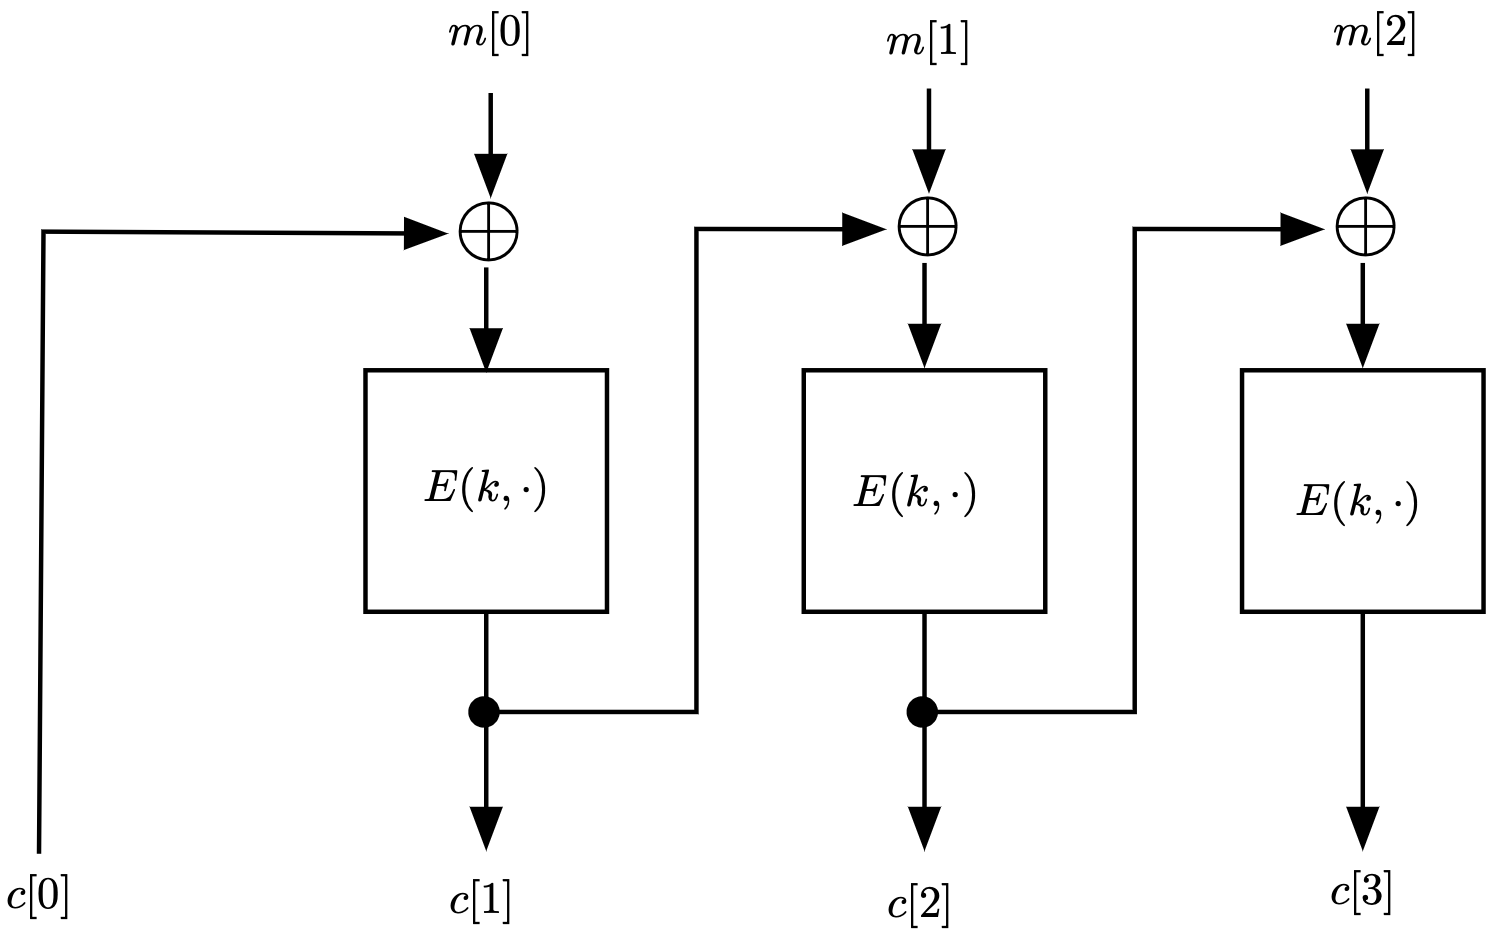
\includegraphics[width=0.65\linewidth]{figures/chapter5/fig4-a.png}}

  \subfigure[解密]{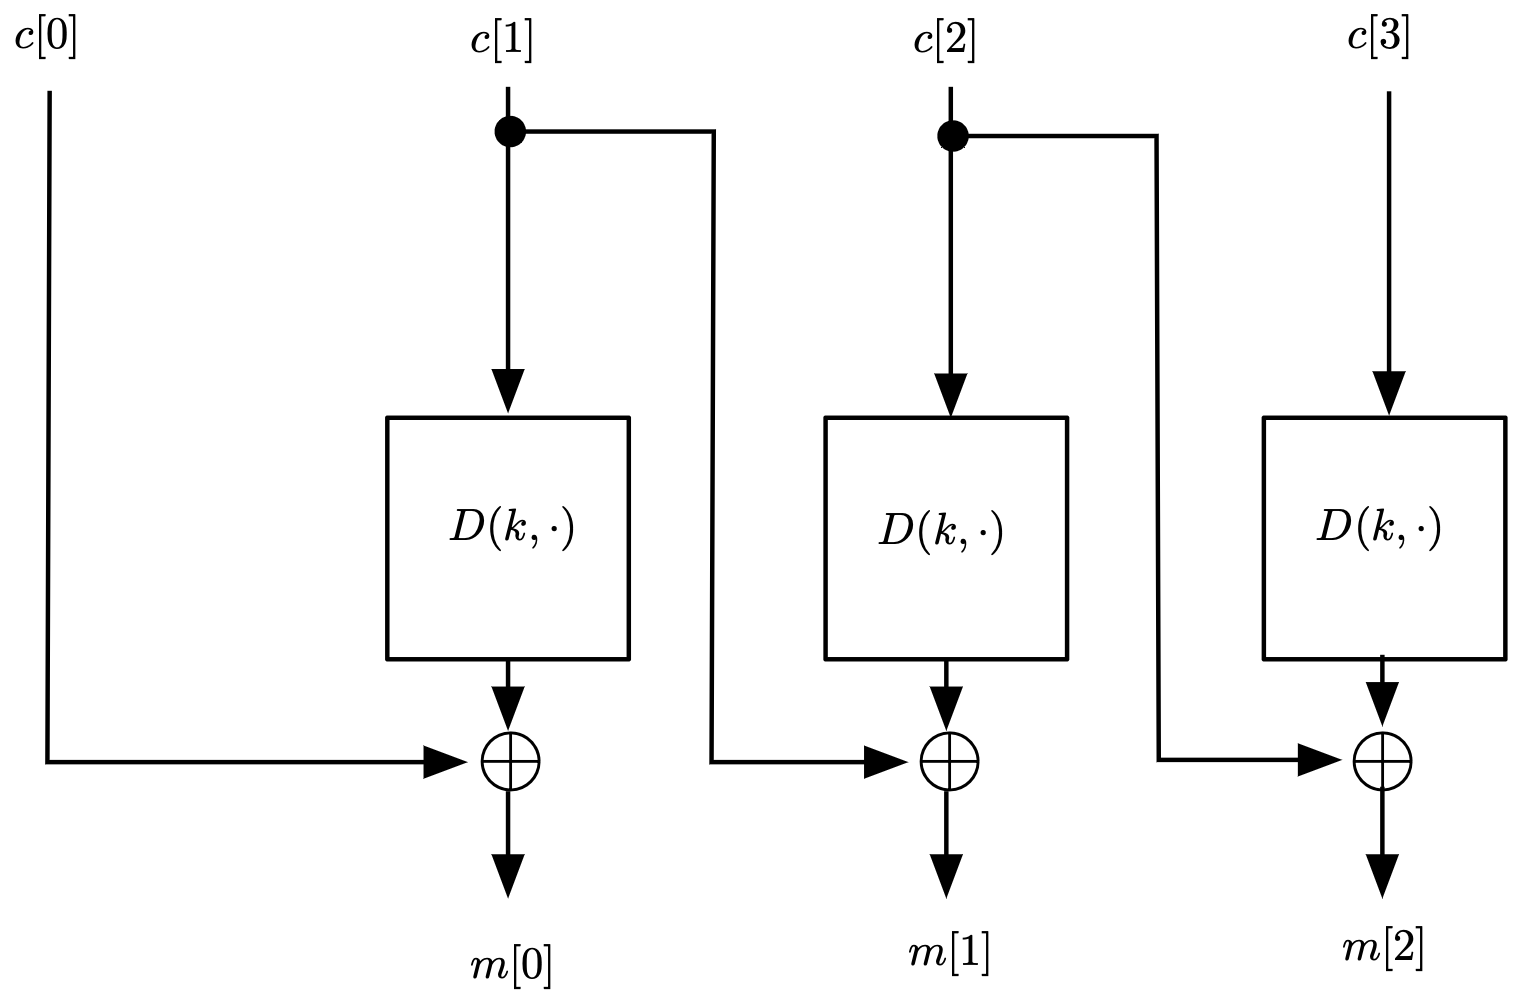
\includegraphics[width=0.65\linewidth]{figures/chapter5/fig4-b.png}}
  \caption{$\ell=3$时CBC模式的加密和解密}
  \label{fig:5-4}
\end{figure}

\begin{theorem}\label{theo:5-4}
如果 $\mathcal{E}=(E,D)$ 是一个定义在 $(\mathcal{K},\mathcal{X})$ 上的安全的分组密码,并且 $N:=|\mathcal{X}|$ 是超多项式的,那么对于任何多项式约束的 $\ell\geq1$,上面描述的密码 $\mathcal{E}'$ 都是一个 CPA 安全的密码。
\begin{quote}
特别地,对于每一个如攻击游戏 \ref{game:5-2} 的比特猜测版本中那样攻击 $\mathcal{E}'$ 的 CPA 对手 $\mathcal{A}$,如果它最多能向其挑战者发起 $Q$ 次查询,则必然存在一个如攻击游戏 \ref{game:4-1} 中那样攻击 $\mathcal{E}$ 的 BC 对手 $\mathcal{B}$,其中 $\mathcal{B}$ 是一个围绕 $\mathcal{A}$ 的基本包装器,满足:
\end{quote}
\begin{equation}\label{eq:5-22}
{\rm CPA}\mathsf{adv}[\mathcal{A},\mathcal{E}']\leq\frac{2Q^2\ell^2}{N}+2\cdot{\rm BC\mathsf{adv}}[\mathcal{B},\mathcal{E}]
\end{equation}
\end{theorem}

\begin{proof}[证明思路]
证明的基本思路与定理 \ref{theo:5-3} 非常相似。我们从一个对 $\mathcal{E}'$ 进行 CPA 攻击游戏的对手开始,然后用一个真随机函数 $f$ 代替 $\mathcal{E}$。然后我们论证,挑战者两次使用同一输入值评估 $f$ 的概率是可忽略不计的。这样一来,挑战者看到的只是一堆随机比特,因此根本无法了解到关于加密消息的信息。
\end{proof}

\begin{proof}
假设 $\mathcal{A}$ 是一个有效的 CPA 对手,它按照攻击游戏 \ref{game:5-2} 攻击 $\mathcal{E}'$,且在该游戏中最多向其挑战者发起 $Q$ 次查询。我们想证明,如果 $\mathcal{E}$ 是一个安全的分组密码,并且 $N$ 是超多项式的,则 ${\rm CPA}\mathsf{adv}^*[\mathcal{A},\mathcal{E}]$ 是可忽略不计的。基于这些假设,根据推论 \ref{cor:4-5},加密函数 $E$ 是定义在 $(\mathcal{K},\mathcal{X},\mathcal{X})$ 上的一个安全的 PRF。

不妨使用攻击游戏 \ref{game:5-2} 的比特猜测版本。我们需要证明,对于一个有效对手 $\mathcal{B}$,有:
\begin{equation}\label{eq:5-23}
{\rm CPA}\mathsf{adv}^*[\mathcal{A}, \mathcal{E}']\leq\frac{Q^2\ell^2}{N}+{\rm BC\mathsf{adv}}[\mathcal{B},\mathcal{E}]
\end{equation}
那么式 \ref{eq:5-22} 就可由式 \ref{eq:5-4} 得到。

和之前一样,我们定义一连串的游戏:游戏 $0$,游戏 $1$,游戏 $2$ 和游戏 $3$。这些游戏都是在 $\mathcal{A}$ 和不同的挑战者之间进行的。游戏 $0$ 中的挑战者就是攻击游戏 \ref{game:5-2} 的比特猜测版本中就 $\mathcal{E}'$ 的挑战者。在每个游戏中,我们用 $b$ 表示挑战者随机选择的比特,用 $\hat b$ 表示 $\mathcal{A}$ 输出的比特。我们想要证明,对于 $j = 1,\dots,3$,$|\Pr[W_j]-\Pr[W_{j-1}]|$ 的值都可忽略不计;此外,$\Pr[W_3]={1}/{2}$ 是显然成立的,于是我们可以得到 ${\rm CPA}\mathsf{adv}^*[\mathcal{A}, \mathcal{E}']:=|\Pr[W_0]-{1}/{2}|$ 也可忽略不计。

\vspace{5pt}

\noindent\textbf{游戏$\mathbf{0}$}。
我们可以将游戏 $0$ 中的挑战者描述如下:

\vspace{5pt}

\hspace*{5pt} 选取 $b\overset{\rm R}\leftarrow\{0,1\}$\\
\hspace*{26pt} 选取 $k'\overset{\rm R}\leftarrow\mathcal{K}$\\
\hspace*{26pt} 当收到第 $i$ 个查询 $(m_{i0},m_{i1})$ 时,记 $v_i:=|m_{i0}|=|m_{i1}|$:\\
\hspace*{50pt} 按如下方法计算 $c_i\in\mathcal{X}^{v_i+1}$:\\
\hspace*{75pt} 选取 $c_i[0]\overset{\rm R}\leftarrow\mathcal{X}$\\
\hspace*{75pt} 对于 $j=0,\dots,v_i-1$:\\
\hspace*{100pt} 计算 $x_{ij}\leftarrow c_i[j]\oplus m_{ib}[j]$\\
\hspace*{100pt} 令 $c_i[j+1]\leftarrow E(k,x_{ij})$\\
\hspace*{50pt} 将 $c_i$ 发送给对手。

\vspace{5pt}

根据构造,我们有:
\begin{equation}\label{eq:5-24}
{\rm CPA}\mathsf{adv}^*[\mathcal{A},\mathcal{E}']= |\Pr[W_0]-{1}/{2}|
\end{equation}


\noindent\textbf{游戏$\mathbf{1}$}。
接下来,我们打出``PRF牌",用一个真随机函数 $f\in{\rm Funs}[\mathcal{X},\mathcal{X}]$ 代替 $F(k,\cdot)$。我们的挑战者在该游戏中看起来是这样的:

\vspace{5pt}

\hspace*{5pt} 选取 $b\overset{\rm R}\leftarrow\{0,1\}$\\
\hspace*{26pt} 选取 $f\overset{\rm R}\leftarrow{\rm Funs}[\mathcal{X},\mathcal{X}]$\\
\hspace*{26pt} 当收到第 $i$ 个查询 $(m_{i0},m_{i1})$ 时,记 $v_i:=|m_{i0}|=|m_{i1}|$:\\
\hspace*{50pt} 按如下方法计算 $c_i\in\mathcal{X}^{v_i+1}$:\\
\hspace*{75pt} 选取 $c_i[0]\overset{\rm R}\leftarrow\mathcal{X}$\\
\hspace*{75pt} 对于 $j=0,\dots,v_i-1$:\\
\hspace*{100pt} 计算 $x_{ij}\leftarrow c_i[j]\oplus m_{ib}[j]$\\
\hspace*{100pt} 令 $c_i[j+1]\leftarrow f(x_{ij})$\\
\hspace*{50pt} 将 $c_i$ 发送给对手。

\vspace{5pt}

我们声称:
\begin{equation}\label{eq:5-25}
|\Pr[W_1]-\Pr[W_0]|={\rm PRF}\mathsf{adv}[\mathcal{B},E]
\end{equation}
其中 $\mathcal{B}$ 是一个有效 PRF 对手;此外,由于我们假设 $F$ 是一个安全的 PRF,且 $N$ 是超多项式的,所以 ${\rm PRF}\mathsf{adv}[\mathcal{B},E]$ 一定是可忽略不计的。希望这(目前)已经是一个常规的论证,我们把具体的论证细节留给读者自行完成。

\vspace{5pt}

\noindent\textbf{游戏$\mathbf{2}$}。
相信读者应该已经知道我们下一步想要干什么了:我们用一个``忠实的侏儒"来实现随机函数 $f$。为此,我们引入一个随机值 $y_{ij}$ 来作为 $c_i[j]$ 的``默认"值,但如果有必要的话,这个值也可以被覆写,就像标有 ($*$) 的那一行所示:

\vspace{5pt}

\hspace*{5pt} 选取 $b\overset{\rm R}\leftarrow\{0,1\}$\\
\hspace*{26pt} 对于 $i=1,\dots,Q$ 和 $j=0,\dots,\ell$:\\
\hspace*{50pt} 设置 $y_{ij}\overset{\rm R}\leftarrow\mathcal{X}$\\
\hspace*{26pt} 当收到第 $i$ 个查询 $(m_{i0},m_{i1})$ 时,记 $v_i:=|m_{i0}|=|m_{i1}|$:\\
\hspace*{50pt} 按如下方法计算 $c_i\in\mathcal{X}^{v_i+1}$:\\
\hspace*{75pt} 选取 $c_i[0]\leftarrow y_{i0}$\\
\hspace*{75pt} 对于 $j=0,\dots,v_i-1$:\\
\hspace*{100pt} 计算 $x_{ij}\leftarrow c_i[j]\oplus m_{ib}[j]$\\
\hspace*{100pt} 令 $c_i[j+1]\leftarrow y_{i(j+1)}$\\
\hspace*{3pt} ($*$)
\hspace*{76.5pt} 如果存在某个 $(i',j')<(i,j)$ 使得 $x_{ij}'=x_{i'j'}$,则令 $c_i[j+1]\leftarrow c_{i'}[j'+1]$\\
\hspace*{50pt} 将 $c_i$ 发送给对手。

\vspace{5pt}

我们显然有:
\begin{equation}\label{eq:5-26}
\Pr[W_2]=\Pr[W_1]
\end{equation}

\noindent\textbf{游戏$\mathbf{3}$}。
接下来,我们让我们的侏儒变得``健忘",只需要丢掉标有 ($*$) 的那一行中的检查:

\vspace{5pt}

\hspace*{5pt} 选取 $b\overset{\rm R}\leftarrow\{0,1\}$\\
\hspace*{26pt} 对于 $i=1,\dots,Q$ 和 $j=0,\dots,\ell$:\\
\hspace*{50pt} 设置 $y_{ij}\overset{\rm R}\leftarrow\mathcal{X}$\\
\hspace*{26pt} 当收到第 $i$ 个查询 $(m_{i0},m_{i1})$ 时,记 $v_i:=|m_{i0}|=|m_{i1}|$:\\
\hspace*{50pt} 按如下方法计算 $c_i\in\mathcal{X}^{v_i+1}$:\\
\hspace*{75pt} 选取 $c_i[0]\leftarrow y_{i0}$\\
\hspace*{75pt} 对于 $j=0,\dots,v_i-1$:\\
\hspace*{100pt} 计算 $x_{ij}\leftarrow c_i[j]\oplus m_{ib}[j]$\\
\hspace*{100pt} 令 $c_i[j+1]\leftarrow y_{i(j+1)}$\\
\hspace*{50pt} 将 $c_i$ 发送给对手。

\vspace{5pt}

为了分析 $|\Pr[W_3]-\Pr[W_2]|$ 的值,我们使用差分引理(定理 \ref{theo:4-7})。为此,我们将游戏 $2$ 和游戏 $3$ 视为运行在相同的基础概率空间上:对手和挑战者所做的随机选择在两个游戏中都是相同的,仅有的不同是挑战者计算应答的规则。

我们定义 $Z$ 为存在 $x_{ij}'=x_{i'j'}$ 在游戏 $3$ 中成立的事件。注意到,事件 $Z$ 是以游戏 $3$ 中的 $x_{ij}$ 值来定义的。事实上,$x_{ij}$ 的值在游戏 $2$ 和游戏 $3$ 中的计算方式可能不一样,所以我们明确地以游戏 $3$ 中的值来定义事件 $Z$。显然,除非 $Z$ 发生,否则游戏 $2$ 和游戏 $3$ 的流程是相同的;特别是,当且仅当 $W_3\land\bar{Z}$ 发生时,$W_2\land\bar{Z}$ 才会发生。因此,基于差分引理,我们有:
\begin{equation}\label{eq:5-27}
|\Pr[W_3]-\Pr[W_2]|\leq\Pr[Z]
\end{equation}

我们声称:
\begin{equation}\label{eq:5-28}
\Pr[Z]\leq\frac{Q^2\ell}{2N}
\end{equation}
为了证明这一点,我们用 $Coins$ 来表示 $\mathcal{A}$ 做出的随机选择。观察到在游戏 $3$ 中,下面的几个值:
\[
Coins,\quad
b,\quad
y_{ij}\;(i=1,\dots,Q,\;j=0,\dots,\ell)
\]
是独立分布的。

考虑任意固定索引 $i=1,\dots,Q$。我们以 $Coins$,$b$ 和 $y_{i'j}$ 的任意固定值作为条件,其中 $i'=1,\dots,i-1$,$j=0,\dots,\ell$。在这个条件概率空间中,$m_{i0}$,$m_{i1}$ 和 $v_i$ 的值是完全确定的,对于 $i'=1,\dots,i-1$ 和 $j=0,\dots,v_{i'-1}$,$v_{i'}$ 和 $x_{i'j}$ 的值也是如此。然而,$y_{i0},\dots,y_{i\ell}$ 的值仍独立且均匀地分布在 $\mathcal{X}$ 上。此外,因为对于 $j=0,\dots,v_i-1$,我们有 $x_{ij}=y_{ij}\oplus m_{ib}[j]$,可知这些 $x_{ij}$ 也均匀独立分布在 $\mathcal{X}$ 上。因此,对于任意固定索引 $j=0,\dots,v_i-1$ 以及满足 $(i',j')<(i,j)$ 的固定索引 $i'$ 和 $j'$,$x_{ij}=x_{i'j'}$ 在上述条件概率空间中成立的概率为 ${1}/{N}$。因此,我们就可以通过一个简单的计算得到式 \ref{eq:5-28}。

最后,我们声称:
\begin{equation}\label{eq:5-29}
\Pr[W_3]={1}/{2}
\end{equation}
这是因为:
\[
Coins,\quad
b,\quad
y_{ij}\;(i=1,\dots,Q,\;j=0,\dots,\ell)
\]
是独立分布的,且对手的输出 $\hat{b}$ 是:
\[
Coins,\quad
y_{ij}\;(i=1,\dots,Q,\;j=0,\dots,\ell)
\]
的一个函数。由此我们可以看到,$\hat b$ 和 $b$ 是相互独立的,于是我们立即就可以得到式 \ref{eq:5-29}。

将式 \ref{eq:5-24} 和式 \ref{eq:5-29} 结合,我们就有:
\[
{\rm CPA}\mathsf{adv}^*[\mathcal{A}, \mathcal{E}']\leq\frac{Q^2\ell^2}{2N}+{\rm PRF\mathsf{adv}}[\mathcal{B},E]
\]
根据定理 \ref{theo:4-4},我们有:
\[
\big\lvert
{\rm BC\mathsf{adv}}[\mathcal{B},\mathcal{E}]-{\rm PRF\mathsf{adv}}[\mathcal{B},E]
\big\rvert
\leq\frac{Q^2\ell^2}{2N}
\]
这样就可以得到式 \ref{eq:5-23},于是该定理得证。
\end{proof}

\subsection{案例研究:TLS 1.0 中的 CBC 填充法}\label{subsec:5-4-4}

令 $\mathcal{E}=(E,D)$ 是一个领域为 $\mathcal{X}$ 的分组密码。我们对使用 $\mathcal{E}$ 的 CBC 模式加密的描述假定要加密的消息都是$\mathcal{X}^{\leq\ell}$ 中的元素。当领域是 $\mathcal{X}=\{0,1\}^{128}$ 时,就像 AES 的情况那样,这意味着我们只能加密那些长度为 $16$ 字节的倍数的消息。但是如果消息的长度并不是分组大小的整数倍,该怎么办呢?

现在,假设我们想用 CBC 模式的 AES 来加密一个 $v$ 字节的消息 $m$,而 $v$ 不一定是 $16$ 的倍数。我们首先想到的是对 $m$ 进行填充,使其长度为 $16$ 的倍数。显然,填充函数必须是可逆的,这是为了让我我们能在解密过程中移除填充。

TLS 1.0 协议定义了以下填充函数,用于在 CBC 模式下用 AES 加密一个 $v$ 字节的消息:令 $p:=16-(v\;\mathrm{mod}\;16)$,然后将 $p$ 字节的内容附加到消息 $m$ 后,且每个字节的内容都是 $p-1$。比如说,我们现在考虑以下两种情况:
\begin{itemize}
	\item 如果 $m$ 的长度是 $29$ 字节,那么 $p = 3$,此时填充由长度为 $3$ 个字节的消息 ``$222$" 组成,这样,填充后的消息长为 $32$ 字节,正好是两个 AES 分组。
	\item 如果 $m$ 的长度是分组大小的整数倍,比如 $32$ 字节,则 $p = 16$,那么填充就由 $16$ 字节组成。这样,填充后的消息长为 $48$ 字节,也就是三个 AES 分组。
\end{itemize}
即使消息长度是分组长度的整数倍,我们仍然需要在最后添加一个完整的假分组,这看起来好像很奇怪。但这是必要的,因为我们要保证解密程序能够正确地移除填充。基于上述设计,无论消息长度如何,填充方法都是可逆的。

一个很容易证明的事实是,任何 CBC 模式加密的可逆填充方案都要基于一个安全的分组密码,它能够为任意长度的消息提供 CPA 安全性。

只要明文长于一个分组,CBC 模式的填充方案就可以用一种叫做\textbf{密文窃取 (ciphertext stealing)}的方法来避免。我们会在练习 5.16 中讨论密文窃取在CBC下的一个变体。当需要加密的消息短于一个分组长时,比如说单字节的消息,仍然是需要进行填充的。

\subsection{计数器模式和 CBC 模式的比较}\label{subsec:5-4-5}

在本节的最后,我们对计数器模式和 CBC 模式进行一个简单地比较。我们假设计数器模式是用一个 PRF $F$ 实现的,它能将 $n$ 比特分组映射到 $n$ 比特分组,而 CBC 模式是用一个 $n$ 比特的分组密码实现的。在这两种情况下,我们都假设消息空间由最多 $\ell$ 个 $n$ 比特数据分组组成。基于本节给出的几个安全定理,我们有如下约束:
\[
\begin{aligned}
{\rm CPA}\mathsf{adv}[\mathcal{A}, \mathcal{E}_{\rm ctr}]\leq\frac{4Q^2\ell}{2^n}+2\cdot{\rm PRF}\mathsf{adv}[\mathcal{B}_F,F]\\
{\rm CPA}\mathsf{adv}[\mathcal{A},\mathcal{E}_{\rm cbc}]\leq\frac{2Q^2\ell^2}{2^n}+2\cdot{\rm BC}\mathsf{adv}[\mathcal{B}_\mathcal{E},\mathcal{E}]
\end{aligned}
\]
这里,$\mathcal{A}$ 可以是任意向其挑战者发起最多 $Q$ 次查询的 CPA 对手,$\ell$ 是任何一条消息的最大长度(数据分组数量)。出于简化讨论的目的,我们在下面的叙述中会忽略 ${\rm PRF}\mathsf{adv}[\mathcal{B}_F,F]$ 和 ${\rm BC}\mathsf{adv}[\mathcal{B}_\mathcal{E},\mathcal{E}]$ 这两项。

我们立即就可以看到,计数器模式有一个可量化的安全优势。为了更具体的解释这一问题,我们不妨假设分组大小为 $n=128$,每条消息为 1 MB(即 $2^{23}$ 比特),因此 $\ell=2^{16}$ 个分组。如果我们想把对手的优势约束在 $2^{-32}$ 以下,那么对于计数器模式,我们最多可以加密 $Q=2^{39.5}$ 条消息,而对于 CBC 模式,我们最多只能加密 $2^{32}$ 条消息。一旦用一个给定的密钥加密了 $Q$ 条消息之后,我们就必须换一个新的密钥。因此,与 CBC 模式相比,计数器模式中的一个密钥可以用来安全地加密更多的消息。

但是需要注意的是,如果使用一个分组密码来实现 $F$,这种数量上的优势就会消失,因为根据 PRF 切换引理(定理 \ref{theo:4-4})中的误差项,我们此时也需要依赖 $\ell$ 的二次项。然而,对于一个定制的 PRF 来说,这种数量上的优势仍然是适用的。

与 CBC 模式相比,计数器模式还有以下几个优点:
\begin{itemize}
	\item \emph{并行化和流水线}。计数器模式的加解密都是很容易并行化的,而尽管 CBC 模式的解密是可以并行化的,但其加密必然是串行性的。当底层硬件能够并行地处理多条指令时,支持并行地模式能够大大改善性能,而现代处理器通常就是这样的。更重要的是,考虑一个支持流水线的分组密码的一轮的硬件实现,如英特尔对 AES-128 的实现。流水线化使多个加密指令能够在同一时间执行。像计数器模式这样支持并行化的模式能使流水线保持忙碌,而在 CBC 加密中,由于这种模式固有的串行性,流水线在大多时间是没有被充分使用的。因此,如果明文已经被加载到 L1 缓存中,那么英特尔 Haswell 处理器上的计数器模式加密能比 CBC 模式加密快 $7$ 倍左右。
	\item \emph{更短的密文长度}。对于非常短的消息,计数器模式的密文比 CBC 模式的密文要短得多。例如,考虑一个 $1$ 字节的明文(在SSH协议中加密单个按键时产生)。计数器模式的密文只需要一个分组加 $1$ 字节:那一分组为随机 IV,那 $1$ 字节为加密后的明文。相比之下,一个 CBC 密文是两个完整的分组。如果假设分组长度是 $128$ 比特的话,这将会导致每个 CBC 密文都包含 $15$ 个多余的字节。
	\item \emph{只需加密}。CBC 模式同时使用分组密码的加密算法和解密算法,而计数器模式只会使用加密算法,因而可以简化代码实现。
\end{itemize}

\begin{remark}\label{remark:5-4}
随机化计数器模式和 CBC 模式都需要一个随机 IV。一些密码库实际上让上层应用来提供这个 IV。如果上层应用不努力确保 IV 有足够的随机性,就可能会导致很多的问题。比如说,对于计数器模式,有必要使 IV 足够分散,以便相应的间隔不会重叠。事实上,这个属性对于它来说就足够了。然而,对于 CBC 模式,需求就更多了:它还要求 IV 是不可预测的,参见练习 5.13。

把 IV 留给上层应用来提供,实际上是\emph{基于 nonce 加密}的一个例子,我们将在接下来的 \ref{sec:5-5} 节中详细探讨。
\end{remark}